../cictikz/src/cictikz/data/tex/cictikz_preamble.tex

% A typical system power architecture: regulators step VBUS down to
% VBAT, IO and CORE rails, with the loads and their current ranges
% hanging off the rails.

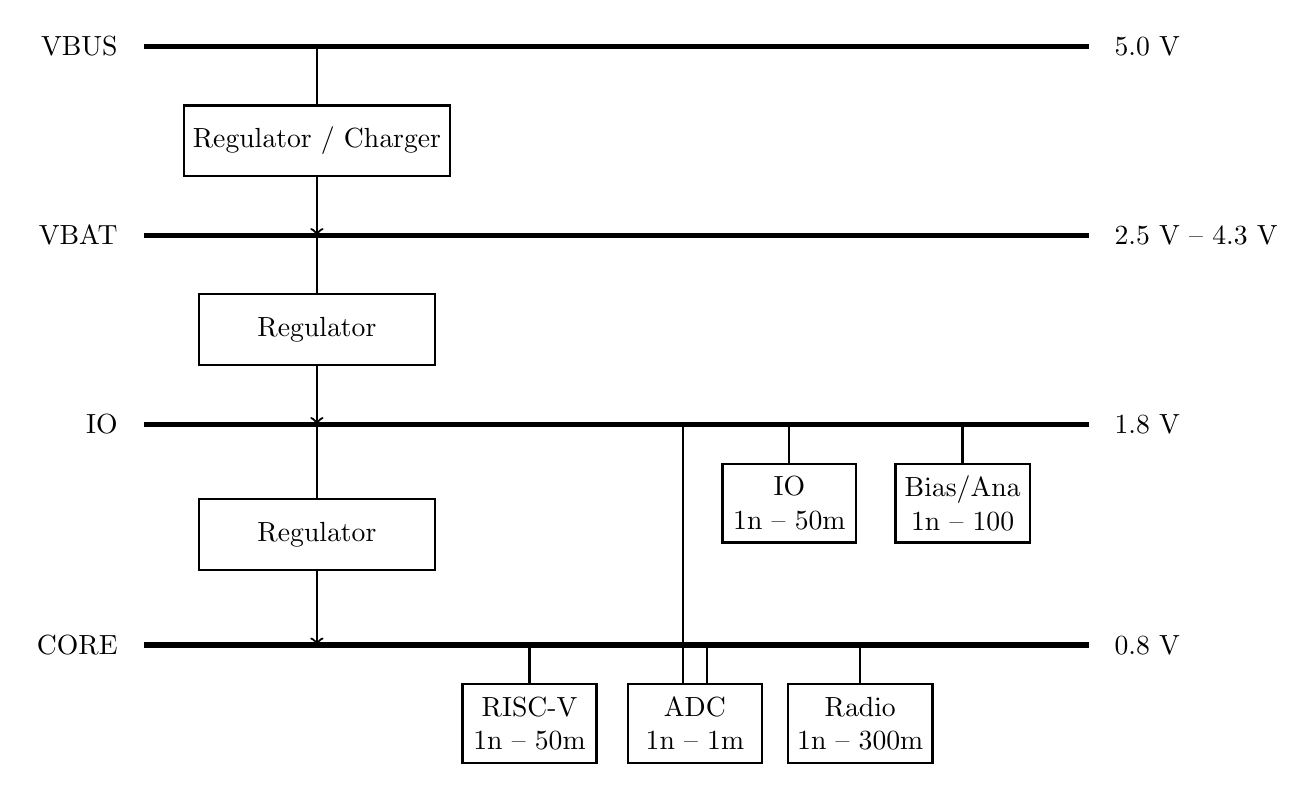
\begin{tikzpicture}[thick,
  reg/.style={draw, rectangle, align=center, minimum width=3.0cm,
              minimum height=0.9cm},
  load/.style={draw, rectangle, align=center, minimum width=1.7cm,
              minimum height=1.0cm},
  a/.style={->}]

  % rails
  \draw[line width=2pt] (0,9.0)  -- (12.0,9.0);
  \draw[line width=2pt] (0,6.6)  -- (12.0,6.6);
  \draw[line width=2pt] (0,4.2)  -- (12.0,4.2);
  \draw[line width=2pt] (0,1.4)  -- (12.0,1.4);

  \node[anchor=east] at (-0.2,9.0) {VBUS};
  \node[anchor=east] at (-0.2,6.6) {VBAT};
  \node[anchor=east] at (-0.2,4.2) {IO};
  \node[anchor=east] at (-0.2,1.4) {CORE};

  \node[anchor=west] at (12.2,9.0) {5.0 V};
  \node[anchor=west] at (12.2,6.6) {2.5 V -- 4.3 V};
  \node[anchor=west] at (12.2,4.2) {1.8 V};
  \node[anchor=west] at (12.2,1.4) {0.8 V};

  % regulators between the rails
  \node[reg] (rc)  at (2.2,7.8) {Regulator / Charger};
  \draw (2.2,9.0) -- (rc.north);
  \draw[a] (rc.south) -- (2.2,6.6);

  \node[reg] (r1) at (2.2,5.4) {Regulator};
  \draw (2.2,6.6) -- (r1.north);
  \draw[a] (r1.south) -- (2.2,4.2);

  \node[reg] (r2) at (2.2,2.8) {Regulator};
  \draw (2.2,4.2) -- (r2.north);
  \draw[a] (r2.south) -- (2.2,1.4);

  % loads on the IO rail
  \node[load] (io)   at (8.2,3.2)  {IO\\1n -- 50m};
  \draw (8.2,4.2) -- (io.north);
  \node[load] (bias) at (10.4,3.2)  {Bias/Ana\\1n -- 100$\upmu$};
  \draw (10.4,4.2) -- (bias.north);

  % loads on the CORE rail
  \node[load] (cpu)   at (4.9,0.4) {RISC-V\\1n -- 50m};
  \draw (4.9,1.4) -- (cpu.north);
  % the ADC hangs on CORE, and also needs the IO rail
  \node[load] (adc)   at (7.0,0.4) {ADC\\1n -- 1m};
  \draw (7.15,1.4) -- (7.15,0.9);
  \draw (6.85,4.2) -- (6.85,0.9);
  \node[load] (radio) at (9.1,0.4) {Radio\\1n -- 300m};
  \draw (9.1,1.4) -- (radio.north);

\end{tikzpicture}
\end{document}
